\documentclass[tikz,border=8pt]{standalone}
% Shared look for every TikZ diagram. Load with \input{../../tools/tikz-style.tex}
\usepackage[T1]{fontenc}
\usepackage{lmodern}
\renewcommand{\sfdefault}{lmr}  % diagrams use the same serif as the text
\usetikzlibrary{arrows.meta, positioning, shapes.geometric, calc, fit, backgrounds}
\definecolor{cblue}{HTML}{4C78A8}
\definecolor{corange}{HTML}{F58518}
\definecolor{cgreen}{HTML}{54A24B}
\definecolor{cred}{HTML}{E45756}
\definecolor{cpurple}{HTML}{B279A2}
\definecolor{cgrey}{HTML}{6B6B6B}
\tikzset{
  every picture/.style={font=\sffamily, line width=1.2pt},
  box/.style={draw=#1, fill=#1!12, rounded corners=4pt, align=center, inner sep=7pt, minimum height=1.1cm},
  box/.default=cgrey,
  arrow/.style={-{Stealth[length=3mm]}, draw=cgrey, line width=1.4pt},
  title/.style={font=\sffamily\bfseries\Large},
  note/.style={font=\sffamily\small, text=cgrey, align=center},
}
\AtBeginDocument{\hyphenpenalty=10000 \exhyphenpenalty=10000}

% PCA read off the thin SVD of the centred data matrix.
\begin{document}
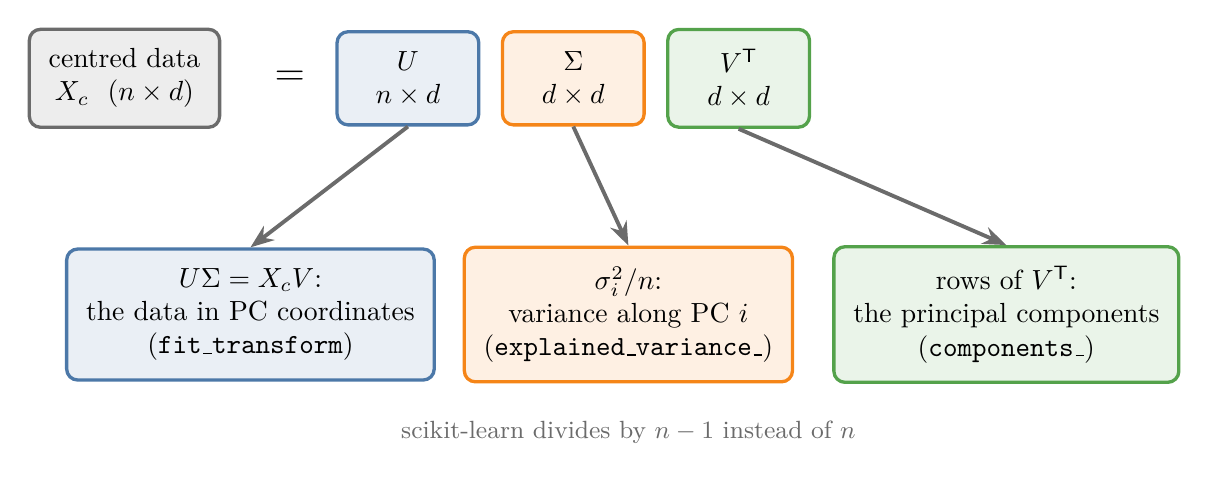
\begin{tikzpicture}
  \node[box=cgrey] (x) at (0,0) {centred data\\ $X_c$ \ ($n \times d$)};
  \node[font=\Large] at (2.1,0) {$=$};
  \node[box=cblue, minimum width=1.8cm] (u) at (3.6,0) {$U$\\ $n \times d$};
  \node[box=corange, minimum width=1.8cm] (s) at (5.7,0) {$\Sigma$\\ $d \times d$};
  \node[box=cgreen, minimum width=1.8cm] (v) at (7.8,0) {$V^{\mathsf T}$\\ $d \times d$};
  \node[box=cblue] (scores) at (1.6,-3) {$U\Sigma = X_cV$:\\ the data in PC coordinates\\ (\texttt{fit\_transform})};
  \node[box=corange] (var) at (6.4,-3) {$\sigma_i^2 / n$:\\ variance along PC $i$\\ (\texttt{explained\_variance\_})};
  \node[box=cgreen] (pc) at (11.2,-3) {rows of $V^{\mathsf T}$:\\ the principal components\\ (\texttt{components\_})};
  \draw[arrow] (u.south) -- (scores.north);
  \draw[arrow] (s.south) -- (var.north);
  \draw[arrow] (v.south) -- (pc.north);
  \node[note] at (6.4,-4.5) {scikit-learn divides by $n - 1$ instead of $n$};
\end{tikzpicture}
\end{document}
